% -*-cap2.tex-*-
% Este fichero es parte de la plantilla LaTeX para
% la realización de Proyectos Final de Carrera, protegido
% bajo los términos de la licencia GFDL.
% Para más información, la licencia completa viene incluida en el
% fichero fdl-1.3.tex

% Copyright (C) 2009 Pablo Recio Quijano 

\section{Introducción}

El primer paso del diseño de la aplicación será describir los requisitos del
sistema necesarios para poder ejecutar la aplicación, y posteriormente comentaremos las herramientas que se
van a usar para el desarrollo de la aplicación.

\section{Definición de los requisitos del sistema}

Los requisitos hardware y software necesarios para poder ejecutar con soltura la aplicación son los siguientes:

\begin{itemize}
	\item Sistema operativo Microsoft Windows en su versión Windows 7, o sistemas basados en GNU/Linux tales como
		la distribución Ubuntu en su versión 10.04.
	\item Últimas actualizaciones del sistema instaladas, drivers y demás aplicaciones propias del sistema
		configuradas correctamente.
	\item Procesador igual o superior a 1,6 GHz.
	\item Memoria RAM igual o superior a 512 MB.
	\item Tarjeta gráfica con aceleración 3D con un mínimo de 128 MB.
	\item En versiones basadas en Linux, se requieren las siguientes bibliotecas:
		\begin{itemize}
			\item python-pygame.
			\item python-setuptools.
			\item PyOpenGL.
			\item PyOpenGL-accelerate.
		\end{itemize}
	\item Por otro lado, si el sistema está basado en Microsoft Windows, necesitaremos:
		\begin{itemize}
			\item PyGame.
			\item Python.
            \item OpenGL
            \item Gloss.
		\end{itemize}
\end{itemize}

\section{Herramientas utilizadas}

\subsection{Biblioteca gráfica}

Para todo el tema del aspecto gráfico, mis tutores me recomendaron que utilizara las bibliotecas SDL\footnote{Simple
Directmedia Layer}, ya que son unas bibliotecas orientadas al desarrollo de videojuegos con varias particularidades:
\begin{itemize}
    \item Son completas, ya que permiten gestionar operaciones de dibujo en dos dimensiones, efectos de
            sonido y música, carga y gestión de imágenes, subsistemas de control de métodos de entrada,
            etcétera, por lo que contamos con una solución global para desarrollar videojuegos.
    \item Están programadas en C, por lo que se puede esperar un buen rendimiento de las bibliotecas en
            diferentes entornos.
    \item Multiplataforma: es compatible oficialmente con los sistemas Microsoft Windows, GNU/Linux,
            Mac OS y QNX, además de otras arquitecturas y sistemas menos comunes como Sega Dreamcast, Sony PSP,
            WebOS, Google Android o Symbian entre otros.
    \item Tampoco hay que mantener al margen la característica de que cuenta con wrappers a otros lenguajes
            de programación como entre los que se encuentran C++, Ada, C\#, BASIC, Erlang, Lua, Java o Python, por
            lo que nos da bastante libertad para elegir un lenguaje de programación principal.
    \item Publicado bajo licencia LGPL, con todas las ventajas que conlleva.
    \item Y por último no hay que menospreciar que uno de mis tutores emplea SDL a la hora de impartir la asignatura
            de Diseño de Videojuegos de la UCA, y contar con su conocimiento nos ha ayudado a desarrollar más rápidamente
            y solucionar antes nuestros posible problemas.
\end{itemize}

\begin{figure}[h]
  \begin{center}
    
\includegraphics[scale=0.5]{SDL.png}
  \end{center}
  \caption{Logotipo de la biblioteca Simple DirectMedia Layer}
  \label{logo-sdl}
\end{figure}

En este aspecto, la utilización de las biblioteca SDL estaba clara. Potencia, comodidad, multiplataforma y con la posibilidad
de utilizar diferentes lenguajes de programación.\\

\subsection{Lenguaje de programación}

Una vez que tocamos el tema de los lenguajes de programación, entra en escena la problemática sobre qué lenguaje
utilizar. En principio se pensó emplear el lenguaje C++ por dos sencillas razones:

\begin{enumerate}
    \item Por un lado es un lenguaje que hemos aprendido en la carrera, se ha utilizado en varias asignaturas de
            diferentes ramas, con lo cual la comodidad y familiaridad que podemos tener a la hora de programar
            es un punto importante a tener en cuenta.
    \item Tampoco podemos olvidar que, al ser un lenguaje compilado, la velocidad de ejecución que se consigue
            es interesante, y mucho más tratándose de temas como la Inteligencia Artificial (donde puede ser
            necesario un uso intensivo de los recursos del sistema) o el desarrollo de videojuegos (en el que
            la potencia del ordenador repercute en una mejor experiencia del usuario).
\end{enumerate}

Pero hay que detenerse un momento y pensar en la naturaleza del proyecto. Aunque el programa a desarrollar sea un
videojuego, no hay que olvidar que hay diferentes tipos de juegos, que pueden condicionar o influir en nuestra forma
de programarlo. En el caso del dominó, lo primero que debemos tener en cuenta es que el apartado gráfico no va a
requerir de una gran potencia o despliegue de efectos: el dominó es un juego pausado y a diferencia de otros
videojuegos lo importante en este caso es mostrar al usuario la información de la partida de una forma clara y sencilla,
para que el jugador evalúe las posibilidades de acción y actúe en consecuencia.\\

\begin{figure}[h]
  \begin{center}
    
\includegraphics[scale=0.3]{python.png}
  \end{center}
  \caption{Logotipo de Python - Copyright Python Software Foundation}
  \label{logo-python}
\end{figure}

Si tenemos en cuenta estas circunstancias, existen otros lenguajes que también deben entrar en juego,
como por ejemplo \textbf{Python}. Buscando las diferencias, ventajas y desventajas de Python frente a C++,
obtenemos el siguiente listado:

\begin{enumerate}
    \item Python es un lenguaje de programación multiparadigma ya que soporta orientación a objetos,
            programación imperativa y, en menor medida, programación funcional.
    \item Al igual que C++ es multiplataforma, y está publicado con la licencia \textbf{Python Software Foundation
            License}, que es una licencia de software libre permisiva, compatible con la GPL.
    \item La sintaxis de Python es muy clara, simple, expresiva y legible, con lo cual los programas
            desarrollados bajo Python son más sencillos de entender \cite{Pilgrim:2004:DP:983200}.
    \item Python es un lenguaje interpretado, a diferencia de C++ que es compilado. Este aspecto podría suponer una
            desventaja ya que al ser interpretado puede resultar más lento, pero analicemos pausadamente estos
            factores:
        \begin{itemize}
            \item Como ya hemos comentado previamente, nuestra aplicación, aunque se enmarca dentro de las
                    facciones de un videojuego, no requiere de grandes alardes de potencia gráfica como podría
                    suponerse, ya que es un tipo de juego pausado y donde cómo se muestra la información
                    es mucho más importante que la velocidad o los efectos de vídeo e imágenes.
            \item A pesar de ser interpretado, un gran conjunto de las funcionalidades de python --- como bibliotecas o
                    funciones básicas del lenguaje --- están programadas internamente en C, así que podríamos
                    verlo como que estamos utilizando la comodidad de Python sobre la potencia de C, uniendo
                    lo mejor de ambos mundos.
        \end{itemize}
\end{enumerate}

Por otro lado, se consigue la gran ventaja de contar con las bibliotecas PyGame. Pygame es un conjunto de módulos
para Python que permiten la creación de videojuegos en dos dimensiones de una manera sencilla.
Funciona como interfaz de las bibliotecas SDL, y está orientado al manejo de sprites. Las grandes ventajas de PyGame son:
\begin{itemize}
    \item Alta portabilidad entre sistemas -- gracias a lo cual cumplimos con el requisito de funcionamiento bajo
            sistemas Windows y GNU/Linux.
    \item Libre y gratuito, disponible bajo licencia LGPL --- gracias a la cual sería posible incluso lanzar los juegos
            de forma comercial, gratuita, libre o incluso shareware.
    \item Soporta CPUs con varios núcleos, incluye funciones altamente optimizadas y escritas en C o directamente en
            ensamblador, altamente configurable y adaptable al proyecto a desarrollar, muy modular, incluye funciones
            para trabajar con eventos y sonidos, y muchas más funcionalidades que lo hacen idóneo para un proyecto
            de estas características.
\end{itemize}

\subsection{Diseño y estilo visual de interfaces}

El diseño visual que se ha desarrollado para la interfaz se ha creado desde cero, buscando los siguientes objetivos:
\begin{itemize}
    \item Líneas sencillas, minimalistas, sin recargar innecesariamente la pantalla.
    \item Botones grandes, para que sea fácil de utilizar por usuarios de edad avanzada.
    \item Textos con un punto de letra elevado, facilitando la rápida lectura y legibilidad del texto.
\end{itemize}

\begin{figure}[h]
  \begin{center}
    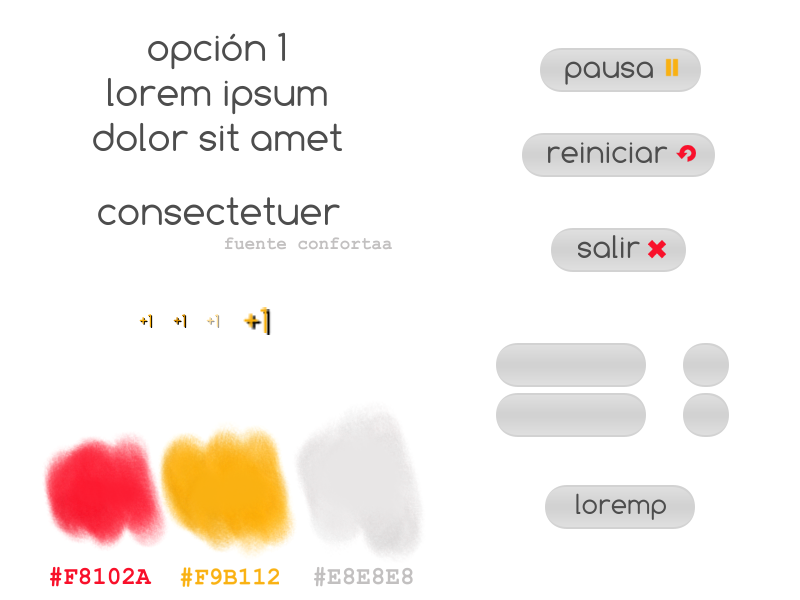
\includegraphics[scale=0.8]{ui.png}
  \end{center}
  \caption{Diferentes elementos utilizados en la interfaz}
  \label{interfaz}
\end{figure}

\subsection{Documentación del código}

Por otro lado, para gestionar toda la documentación del proyecto se decidió utilizar las siguientes herramientas:
\begin{itemize}
    \item \LaTeX\ para escribir la memoria, ya que es una forma robusta y fiable de escribir una memoria para
            un Proyecto Fin de Carrera, descartándose otras posibles opciones por no ser adecuadas para la escritura
            de un documento de estas características~\cite{mitt04}. Para facilitar la compilación dispone de la herramienta
            GNU Make~\cite{pdf:make}.
    \item Doxygen para la documentación del código fuente, porque además de documentar de manera sencilla y fácil
            de leer el mismo código fuente, genera una documentación en diferentes formatos~\cite{website:doxygen}. Además,
            Doxygen funciona con lenguajes como C++, C, Java, Objective-C, Python, Fortran, VHDL, PHP o C\#
            (entre otros), por lo que se puede acomodar a nuestras necesidades. Incluso existe una
            herramienta llamada \textbf{Doxypy} que nos permite reutilizar los comentarios \emph{tipo Python}
            y adaptarlos a Doxygen, con lo cual ahorramos trabajo y cumplimos con la normativa recomendada para el código Python.
\end{itemize}

\subsection{Sistema de control de versiones}

El código del proyecto Dominous, está alojado por completo dentro de
la forja que proporciona Rediris, la Red Española para Interconexión
de los Recursos InformáticoS de las universidades y centros de
investigación, donde tiene su web
oficial~\cite{website:dominous}. Esta forja es básicamente una
instalación de GForge~\cite{website:gforge} con un repositorio
Subversion (SVN) asociado a cada proyecto. \\

Subversion lleva un control exahustivo de todos los ficheros e iteraciones de código que se realizan en él,
permitiendo volver a versiones anteriores de código, comprobar diferencias entre versiones o ficheros y cualquier otra
operación propia de un sistema de control de versiones. \\

Se evaluaron otros sistemas de control de versiones distribuidos como GIT, Bazaar o Mercurial, pero se desecharon
básicamente porque, por un lado, este proyecto cuenta únicamente con un desarrollador, y multitud de ventajas que
ofrecen los sistemas de control de versiones distribuidos dejan de tener sentido. Si tenemos en cuenta esta circunstancia
del proyecto, y por otro lado la integración de SVN con Rediris (con las ventajas de visualización de código y versiones
que ofrece ViewCVS) decantaron la decisión sobre el lado de SVN.

\section{Interfaz gráfica}

Tomando los resultados obtenidos en la fase de análisis es necesario diseñar una interfaz gráfica amigable
para el usuario y desde la cual se pueda interactuar con la aplicación. Para el diseño de las interfaces
se intentará en todo momento que sean usables además de intentar conseguir que el usuario no pueda
introducir datos erróneas para que no produzca comportamientos anómalos.

\begin{figure}[h]
  \begin{center}
    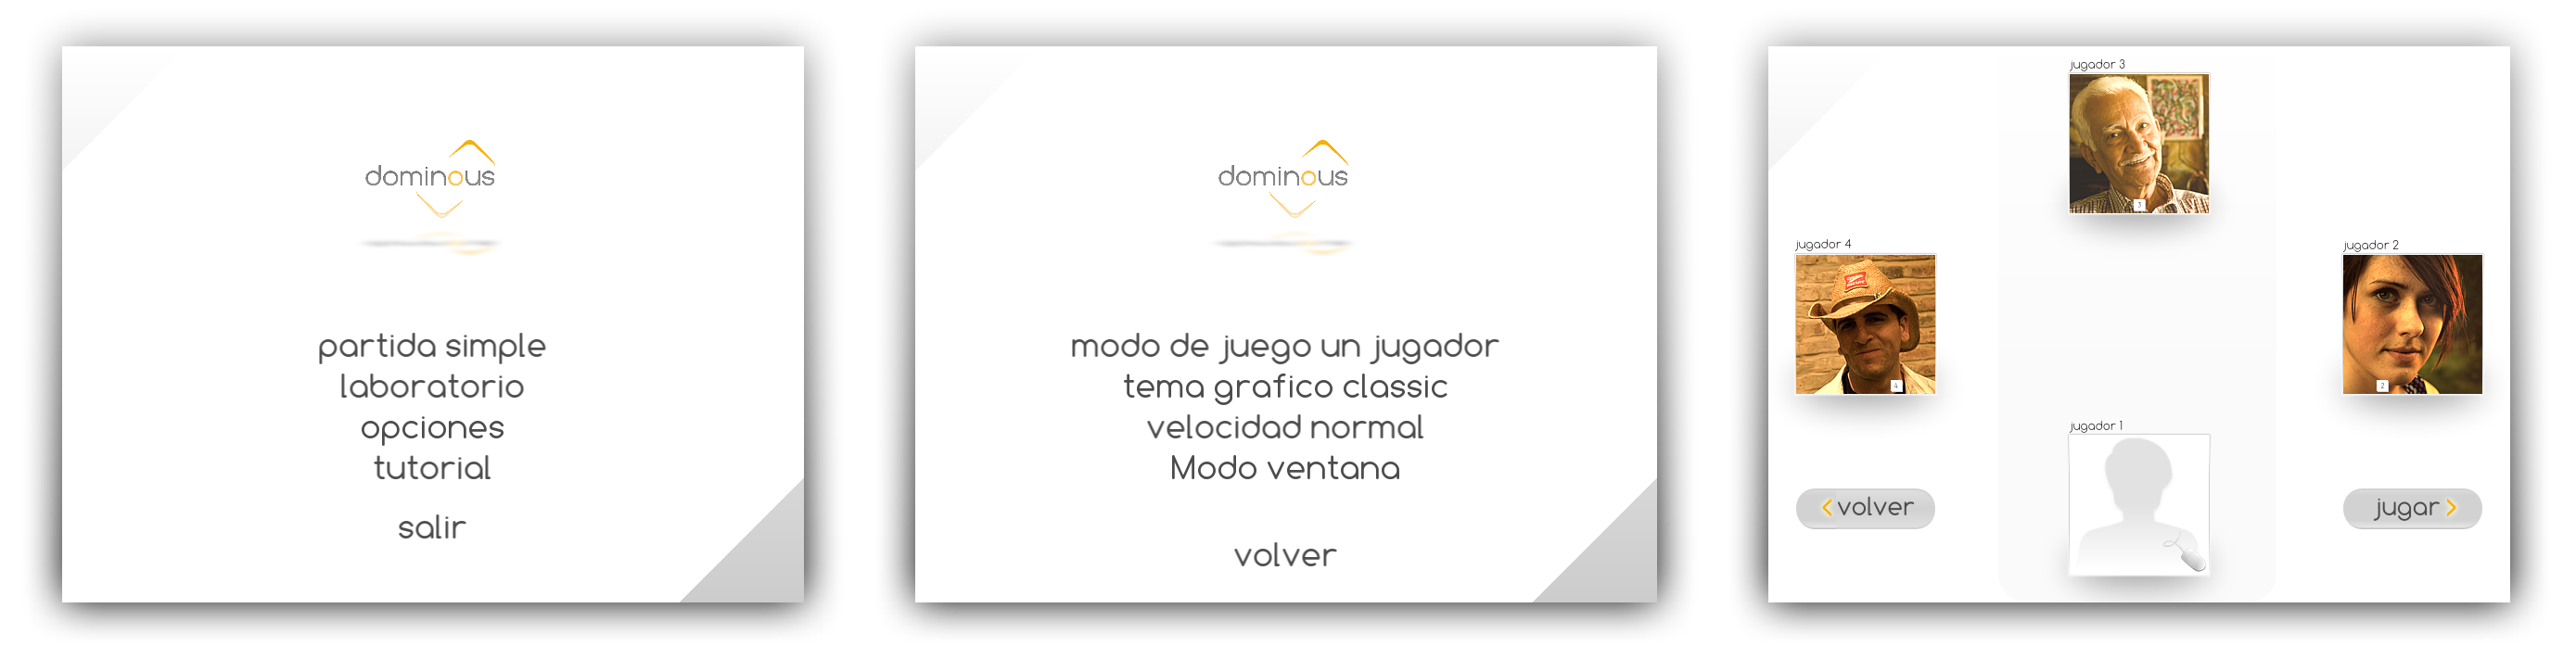
\includegraphics[scale=0.25]{interfaz.png}
  \end{center}
  \caption{Varias pantallas con la interfaz de Dominous}
  \label{fig:pantallas_interfaz}
\end{figure}

\subsection{Diagrama de interacción entre interfaces gráficas}

En el siguiente diagrama~\ref{fig:diagramainteraccioninterfaces} podemos observar la interacción entre
las distintas interfaces gráficas desarrolladas para la aplicación.

\begin{figure}[hp]
  \begin{center}
    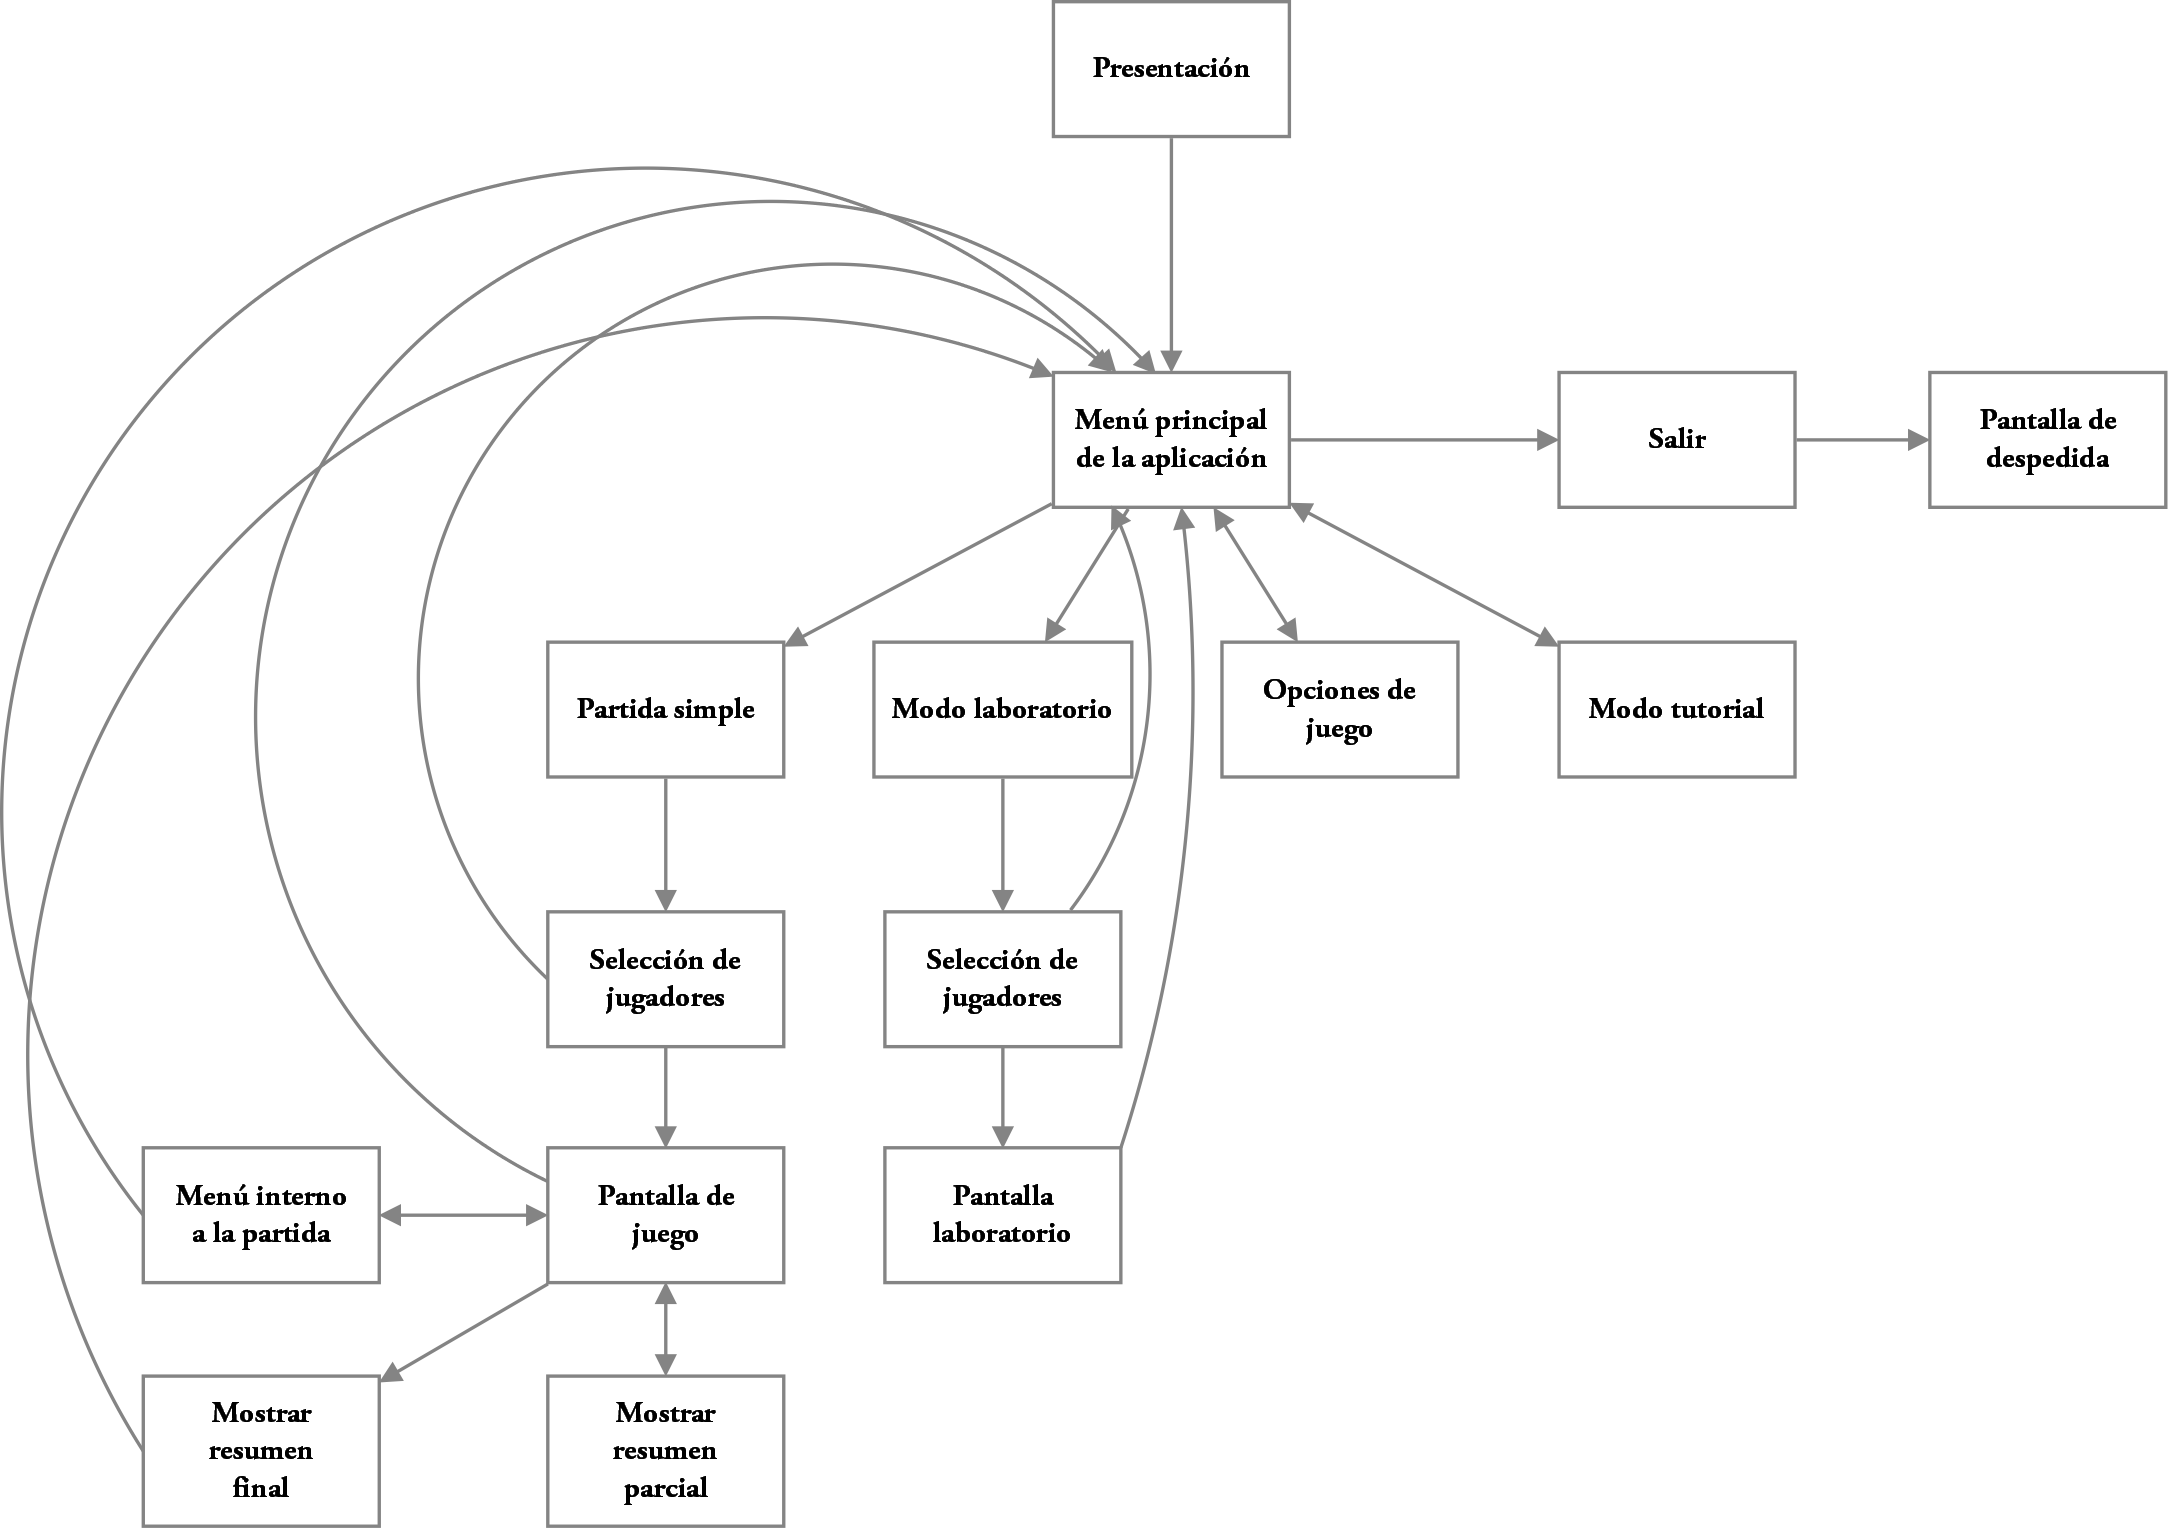
\includegraphics[scale=0.18,angle=90]{diagrama_interfaces.png}
  \end{center}
  \caption{Diagrama de interacción entre interfaces}
  \label{fig:diagramainteraccioninterfaces}
\end{figure}

\section{Diagrama Entidad -- Relación}

La aplicación \textbf{Dominous} realiza un almacenamiento limitado de información, por lo que no se estima necesario
realizar un diagrama Entidad -- Relación con este fin.

\section{Diagrama de clases de diseño}

A continuación se muestra el diagrama de clases de diseño para \textbf{Dominous} (figura~\vref{fig:diagrama_clases_diseno}).

\begin{figure}[hp]
  \begin{center}
    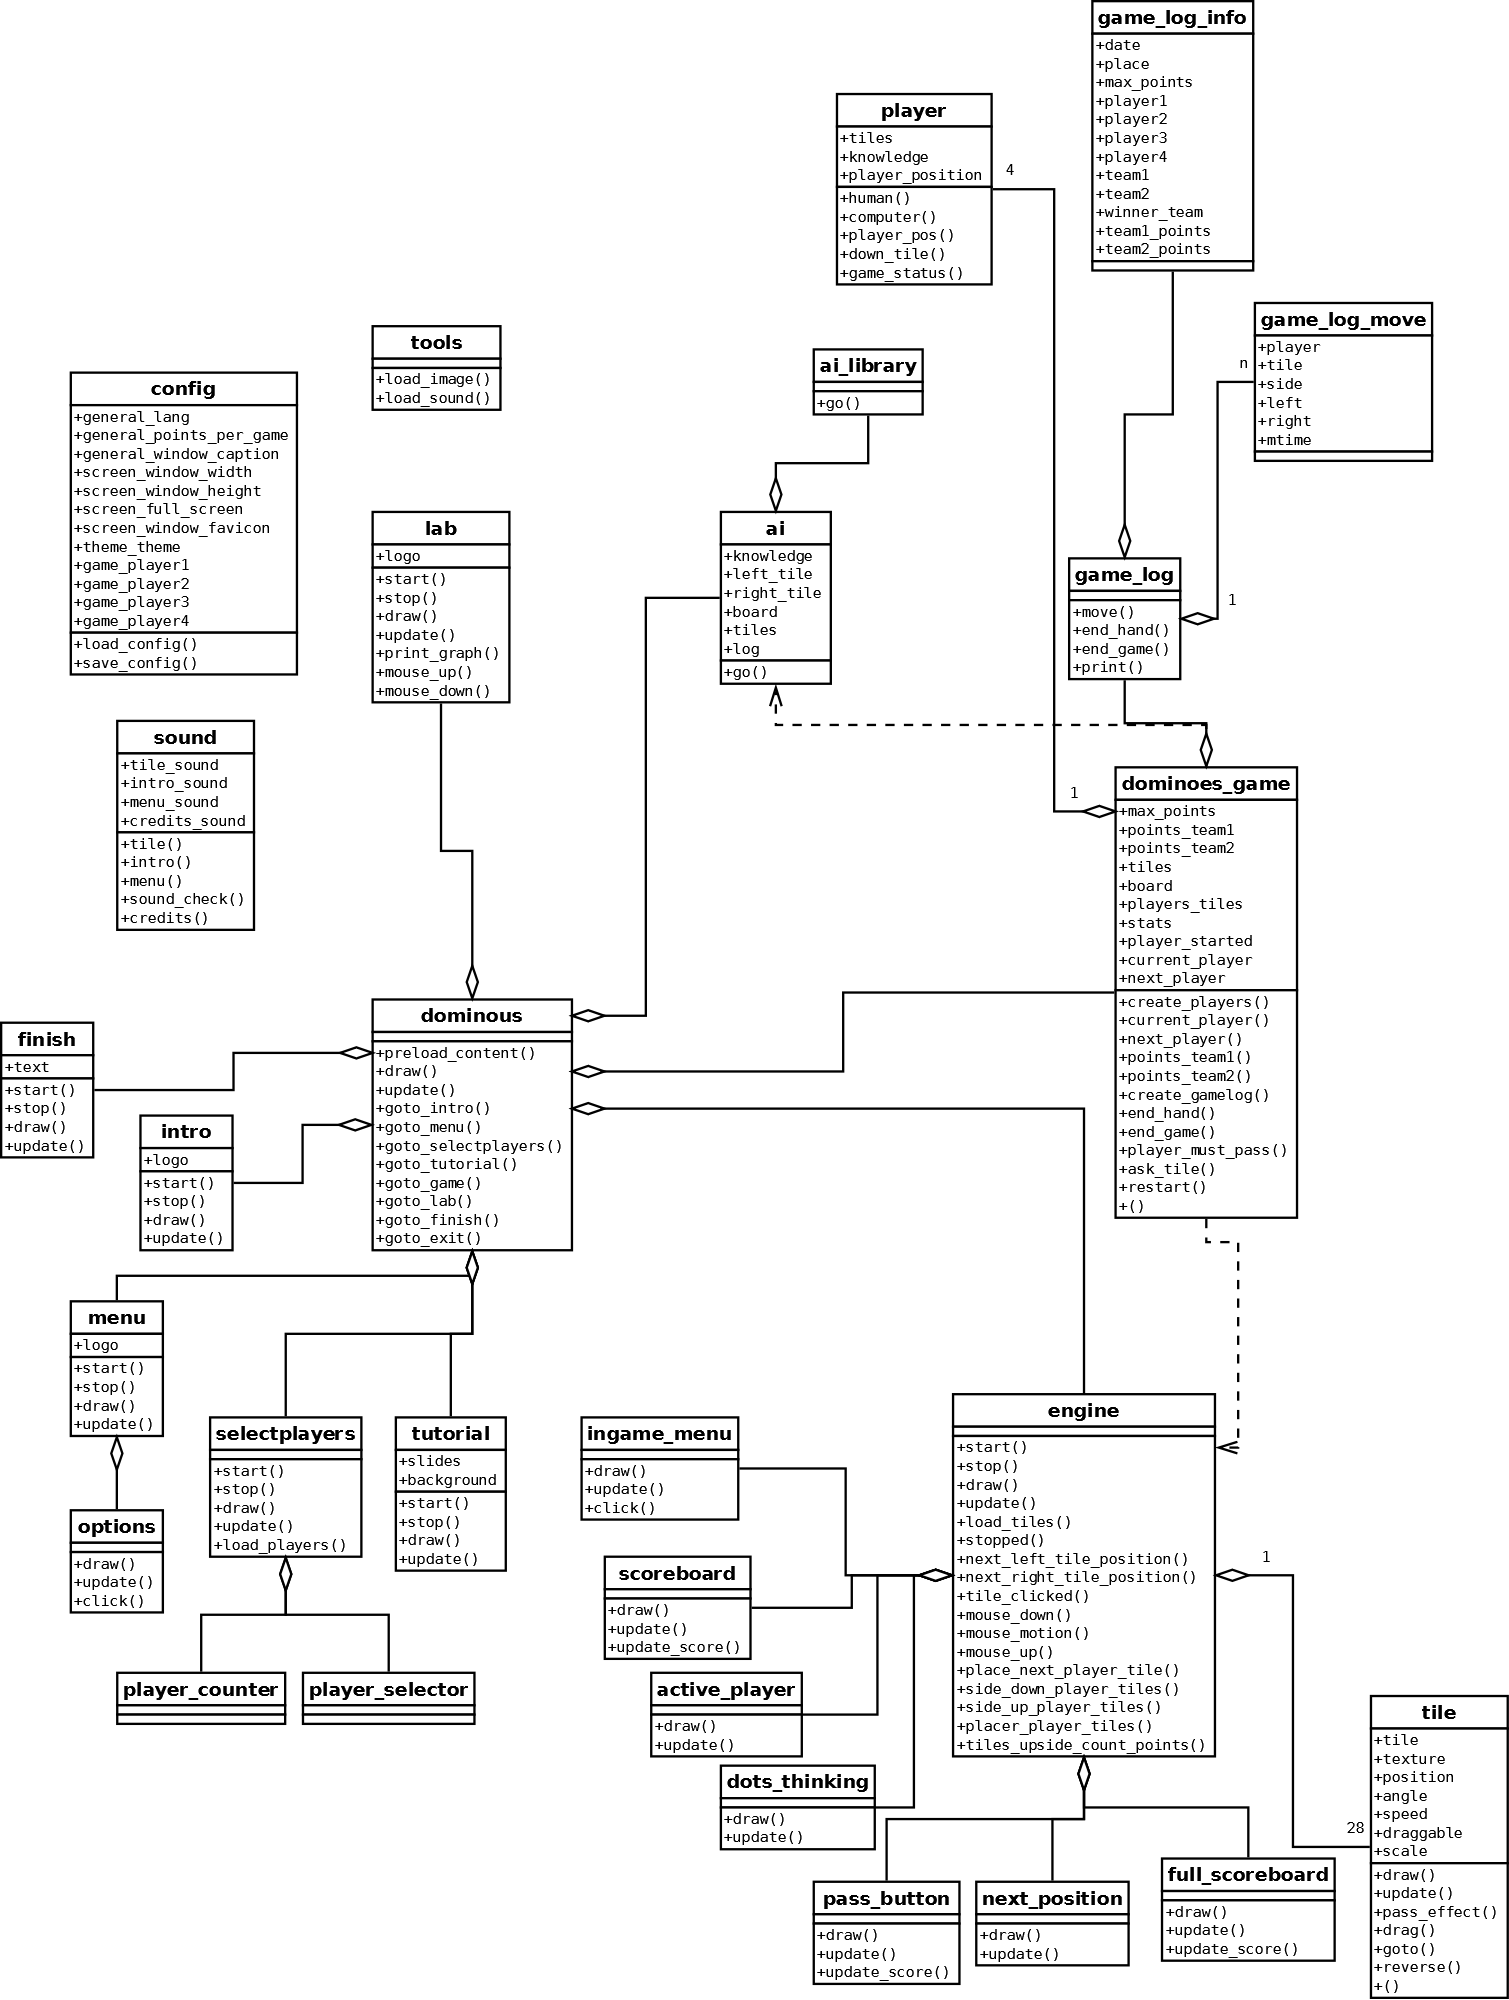
\includegraphics[width=1\textwidth]{diagrama_clases_diseno.png}
  \end{center}
  \caption{Diagrama de diseño del sistema}
  \label{fig:diagrama_clases_diseno}
\end{figure}


\section{Análisis de las principales clases de la aplicación}

En este apartado realizaremos un repaso a las principales clases que intervienen en el diseño de \textbf{Dominous},
definiendo los métodos y atributos que se requieren para el correcto desarrollo de la aplicación y comentando
todos los apartados cuya funcionalidad merezca ser destacada.

\subsection{Clase dominous}

La clase \comando{dominous} genera el objeto principal que soporta el peso principal de toda la aplicación. Al inicio de la
ejecución se crea un objeto de esta clase; este objeto va creando --- según las necesidades del flujo que tome
la ejecución de la misma --- los diferentes objetos, controlando y dando paso a la interfaz activa, llamando a
las principales funciones y permitiendo la captura de los eventos de entrada. \\

Al igual que la gran mayoría de videojuegos, para el desarrollo de Dominous se han utilizado dos métodos principales
que permiten controlar la aplicación en tiempo real. Estos dos métodos son:
\begin{description}
    \item[draw] El primer método se encarga de dibujar en pantalla todos los elementos de la interfaz. El funcionamiento
        básico es recorrer todos los objetos activos y pintarlos según la posición, rotación y escala que tengan en
        ese preciso momento. 
    \item[update] El segundo método se ocupa de realizar los cálculos para el movimiento de los elementos gráficos. 
        En cada iteración cambiará el estado de los objetos activos, modificando la imagen o los valores posición,
        rotación y/o escala, estudiando las posibles colisiones, eventos y cualquier otra circunstancia que cambie
        el estado de la aplicación, para que en el siguiente ciclo se dibujen los elementos en su posición correcta.
\end{description}

Una vez que este objeto principal toma el control de la aplicación, su función es llamar a los métodos \comando{draw}
y \comando{update} del objeto encargado de la interfaz que estemos mostrando actualmente, de forma alternativa. \\

Este juego de llamadas a ambos métodos se realizará hasta un máximo de 60 veces por segundo, dependiendo del rendimiento
que se obtenga de los recursos del sistema. De esta forma conseguiremos un máximo de 60 frames o cuadros por segundo,
que serán los encargados de generar la sensación de movimiento suave. \\

Como vemos, el objeto de la clase dominous no realiza ningún dibujado en pantalla ni cálculos, sino que su único
cometido es redireccionar el flujo de la aplicación al objeto correspondiente.

\subsection{Clase dominoes\_game}

La labor de esta clase es llevar el control de una partida completa de dominó, siguiendo las reglas del \textbf{dominó
internacional}. Dependiendo de la configuración de la partida, creará los jugadores según la selección que se haya
realizado en la pantalla de selección de personajes y comenzará con el bucle principal. \\

Repartirá las fichas entre los diferentes participantes del juego e irá pidiendo fichas a los jugadores de forma
consecutiva, hasta que se de alguna circunstancia de finalización de la mano. \\

Este bucle se repetirá hasta que alguno de los dos equipos alcance o supere los 200 puntos, momento en el cual la partida
se dará por finalizada. \\

Esta clase también mantendrá activo y actualizado un fichero de registro (\emph{log}) con toda la información generada en la partida. Esta
información se utilizará más tarde en el apartado de inteligencia artificial, y almacenará los datos utilizando
la siguiente estructura: \\

Por un lado tenemos la información global de la partida: 

\begin{description}
    \item[date] Fecha de desarrollo de la partida.
    \item[place] Lugar donde tuvo lugar la partida.
    \item[max\_points] Límite superior de puntos necesarios para ganar el encuentro. Como se utilizan las reglas del
        \textbf{dominó internacional}, esta cota estará situada en los doscientos puntos.
    \item[player1] Datos del jugador 1.
    \item[player2] Datos del jugador 2.
    \item[player3] Datos del jugador 3.
    \item[player4] Datos del jugador 4.
    \item[team1] Pareja que forma el equipo 1.
    \item[team2] Pareja que forma el equipo 2.
    \item[points\_team1] Puntos actuales que tiene el equipo 1.
    \item[points\_team2] Puntos actuales que tiene el equipo 2.
    \item[winner\_team] Pareja que finalmente ha sido ganadora de la partida.
\end{description}

Y por otro lado tenemos información relativa a la mano que se está desarrollando actualmente. Esta información se repite
por cada movimiento que se realice en la partida, y se agrupa por manos:

\begin{description}
    \item[player] Jugador que ha realizado el movimiento.
    \item[tile] Ficha que ha colocado.
    \item[side] Lado del tablero por donde ha colocado la ficha.
    \item[left] Cifra, del cero al seis, que se tiene como resultante del movimiento por el lado izquierdo del tablero.
    \item[right] Cifra, del cero al seis, que se tiene como resultante del movimiento por el lado derecho del tablero.
    \item[mtime] Tiempo (en segundos) que ha estado pensando el jugador antes de colocar la ficha.
\end{description}


\section{Sistemas expertos}

Este apartado de la memoria requiere de una especial explicación, ya que a la hora de realizar un videojuego de
dominó goza de gran importancia los diferentes sistemas expertos que participarán en la partida. Estos sistemas expertos,
como bien su nombre indica, simulan el comportamiento de un ser humano experto en una materia, en este caso del juego
de dominó, y su realismo debe hacer sentir al jugador humano que está desempeñando una partida real contra jugadores
también humanos. \\

Enfrentarse a una simulación de inteligencia artificial es una de las empresas más difíciles y complicadas pero a la
vez placenteras y satisfactorias de abarcar en un proyecto de Ingeniería del Software. Los seres humanos utilizan
multitud de métodos y herramientas para razonar y obtener soluciones a problemas concretos, y en muchas ocasiones
este tipo de comportamientos son imposibles de simular, bien por la complejidad computacional que supone, bien por
desconocimiento del funcionamiento exacto que sigue el cerebro para obtener esa solución, o bien por limitaciones de
recursos, ya sea de disco, tiempo de desarrollo o metodologías que simulen ese comportamiento. \\

Por otro lado, aunque el público neófito en la materia pueda suponer que el dominó es un juego de suerte, con un
abanico muy corto de opciones de juego o con una libertad de movimientos muy limitada, nada más lejos de la realidad. \\

El dominó es un juego muy profundo, con normas, técnicas y muchas dosis de psicología, un deporte que obliga al
jugador a estar concentrado al cien por cien durante todo el desarrollo del juego, y un arte con una curva de
aprendizaje poco escarpada, que permite que jugadores nóveles puedan adentrarse en el juego, pero que presenta
mucha complicación convertirse en un gran jugador de dominó. \\

Y, si estas razones que explican la complejidad del mismo no fueran suficientes, no hay más que echarle un vistazo
a los torneos locales o de ámbitos más abiertos para descubrir que las parejas de grandes jugadores sabios y con
una gran compenetración son los que suelen ganar, descartando de forma tajante la posibilidad de que sea la suerte
la que empuje la balanza de la partida hacia un equipo u otro. \\

A la hora de afrontar este problema, el primer paso fue empaparse de cultura y conocimiento sobre el dominó. Las
principales herramientas que se utilizaron fueron:

\begin{description}
    \item[El Libro del dominó] de Benito Ruipérez \cite{mora90}, un libro ameno y profundo sobre el mundo del dominó,
        con multitud de partidas explicadas movimiento a movimiento, trucos, ejemplos, técnicas básicas y avanzadas y
        mucha información.
    \item[Don Manuel Palomo Fernández de Bobadilla] -- jugador amateur de dominó y participante en torneos durante más de cuarenta
        años, con un gran conocimiento de técnicas y métodos de juego, mucha experiencia y una gran facilidad para
        comunicar toda esa sabiduría y conocimiento.
\end{description}

Después de profundizar en el mundo del dominó, y tener cierto conocimiento sobre el mismo podemos intentar definir las pautas sobre
las que va a llevarse a cabo la simulación del sistema experto de dominó. \\

Lo primero que observamos es que la estrategia que siga cada jugador depende enteramente del rol que desempeñe el mismo.
Como vimos en la sección ~\ref{juegoporparejas} es importante definir una estrategia personalizada para cada jugador,
dependiendo del lugar respecto al jugador mano. \\

A continuación mostramos las áreas, campos o ámbitos que debemos tener en cuenta a la hora de resolver con éxito
una partida de dominó.

\subsection{Estrategia según la posición}

Lo primero que observamos es que la estrategia que debe seguir cada jugador depende enteramente del rol que desempeñe el mismo.
Como vimos en la sección ~\ref{juegoporparejas} es importante definir una estrategia personalizada para cada jugador,
dependiendo del lugar respecto al jugador mano, por lo que nuestro sistema debe tener reglas sensibles a esto.

\subsection{Reglas de obligado cumplimiento}

Si leemos el apartado \emph{Normas fundamentales para el juego del dominó por parejas} de \textbf{El Libro del dominó} de
Benito Ruipérez \cite{mora90}, la primera regla que se destaca es la siguiente:

\begin{quote}
    \textbf{Defender el doble del palo iniciado por el compañero} 
\end{quote}
\begin{quote}
    Al iniciar, por obligación, el palo más largo que se lleva, se salga o no, sea o no mano. ¿Cuál ha de ser nuestra
    obligación? Lo más importante para el éxito de este juego es \emph{volver lo primero} (sin excusas ni pretextos)
    la que ha iniciado el compañero, aunque sólo lleves una de ellas, seas mano, te quedes fallo o ambas cosas, no importa.
\end{quote}
\begin{quote}
    Si tu compañero lleva cuatro de doble, como más normal en el dominó, al volverle una de estas, lo has hecho \emph{fuerte}
    en el palo que ha iniciado. Si él ha hecho lo mismo para ti, con otro palo distinto, mandáis en dos palos en
    esa mano: ¿Qué más se puede pedir? El resto de las fichas que lleváis sirve para contrarrestar a los oponentes en sus
    palos largos, y ayudar a que el compañero pueda entrar con el suyo: \emph{vuestros palos fuertes}.
\end{quote}

Como vemos, hay reglas que son de obligado cumplimiento, podríamos decir que \emph{objetivamente} \footnote{Debemos de
reconocer que un recurso válido y muchas veces efectivo a la hora de participar en un juego es utilizar el engaño, pero
como norma general lo evitaremos, ya que también estaríamos engañando a nuestro compañero, pudiendo obtenerse resultados
nefastos.} siempre deben seguirse (sea cual sea la posición del jugador) y, únicamente debemos evitarlas por motivos de
fuerza mayor (ausencia de fichas que nos permitan cumplir esa regla).

\subsection{Pesos de las diferentes reglas}

Comparemos la anterior regla con la siguiente, extraída también de \textbf{El Libro del dominó} \cite{mora90}:

\begin{quote}
    Si el j1 sale con una ficha que no es doble, y el j2 se dobla a una de ellas, el j3 se debe doblar a la otra, si
    lleva el doble, de lo contrario, si no lleva el doble, como la que mate por cualquier lado ha de ser de la
    salida de su compañero, debe poner (cruzar) por el lado de la no doblada.
\end{quote}

Podría decirse que existen diferentes reglas que debemos comprobar si se cumplen, y en caso afirmativo, realizar \emph{la
más importante de ellas}, es decir, con la que consigamos un mayor distanciamiento o ventaja respecto al equipo contrario. \\

Por lo tanto nos vemos en la necesidad de establecer pesos o prioridades a cada una de las reglas que se puedan contemplar
en cada momento, para que la toma de decisiones esté razonada y sea competitiva.

\subsection{Aleatoriedad}

Uno de los problemas que pueden aparecer a la hora de diseñar este sistema experto es la posibilidad de ser predecible. \\

Como vemos, los jugadores posee un conjunto de reglas con prioridades que deben comprobarse y, si se pueden llevar a cabo,
realizar el movimiento descrito en ellas. Esto puede llevar a que, dependiendo de los movimientos que realizan los jugadores,
saber qué fichas poseen (o qué estrategia están siguiendo). \\

Una de las formas de evitar este problema es dotar al sistema de cierta aleatoriedad. Una aleatoriedad que no sea completa,
sino que, para un determinado momento, elija una entre varias de las mejores opciones. Esto se puede simular (e implementar) de forma
sencilla otorgando el mismo peso o prioridad a varias reglas y seleccionando una de ellas. De esta forma los jugadores
humanos no podrán saber ni predecir los movimientos de los jugadores controlados por el ordenador, y el sistema experto
realizará movimientos que pueden ser igual de buenos pero en diferente orden, añadiendo \emph{humanidad} a la programación
de los jugadores.

\subsection{Generación de errores - sistemas imperfectos}

\textbf{Dominous} pretende ser un juego divertido, con el cual aprender a jugar al dominó. Es por ello que una de las
prioridades que se buscan es no crear un sistema que sea imposible de vencer, o que ofrezca una resistencia muy fuerte,
sino un juego que permita adaptar el nivel del jugador humano al de los jugadores manejados por el ordenador. \\

Como vemos, el sistema experto debe permitir dos opciones:
\begin{itemize}
    \item Que los jugadores puedan cometer fallos (simulando por completo el comportamiento de un jugador humano)
    \item O bien que la descripción de las reglas que siga el jugador (o el conjunto de prioridades que se definan
            en las reglas) no sea el adecuado para realizar un juego profesional.
\end{itemize}

Por lo tanto, nuestro sistema experto debe permitir definir cómodamente el conjunto de reglas o los pesos de las mismas.

\subsection{Diferentes jugadores}

Para simplificar y humanizar comportamientos, y representar los diferentes tipos de inteligencias o sistemas expertos,
se ha optado por definir un conjunto de jugadores que se podrán elegir como adversario o pareja a la hora de jugar
una partida de dominó. \\

Cada jugador poseerá unas reglas y unos pesos asociados a esas reglas, con la intención de que el jugador humano pueda
elegir compañeros y adversarios adaptados al nivel concreto que posea el mismo, y de este modo identificamos de forma
sencilla y rápida una \emph{inteligencia} con un avatar definido. \\

Así pues, nuestro sistema debe permitir la generación de diferentes niveles de dificultad o pilas de reglas y pesos,
y asociarlos de forma cómoda a un jugador.

\begin{figure}[h]
  \begin{center}
    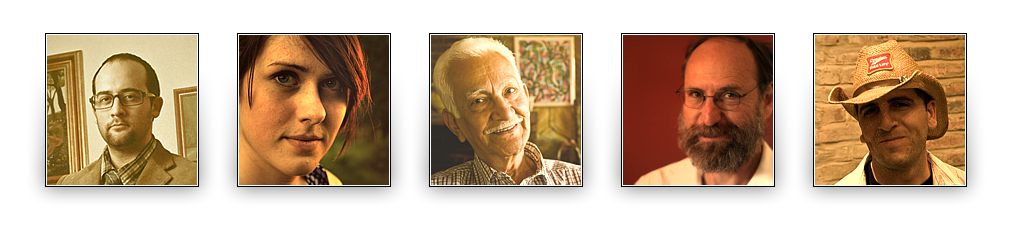
\includegraphics[scale=0.5]{jugadores_dominous.png}
  \end{center}
  \caption{Diferentes imágenes que identifican al conjunto de jugadores de Dominous}
  \label{fig:jugadores_dominous}
\end{figure}

\subsection{Modelado}

Tras realizar un análisis del sistema, se han identificado los siguientes hechos necesarios para que el sistema experto razone:

\begin{description}
    \item[Fichas] Las fichas con las que cuenta el jugador --- en principio todas son posibles candidatas para elaborar
            el movimiento.
    \item[Turno] Dependiendo del turno en que nos encontremos.
    \item[Jugador que manda] Si el jugador que manda es nuestro compañero debemos apoyarle. Si nosotros somos el jugador que
            manda podemos intentar jugar para nosotros.
    \item[Posición del jugador] El lugar del jugador, estimando nuestras posibilidades de victoria.
    \item[Histórico de la partida] En definitiva, se requiere de un histórico con todos los movimientos realizados durante el
            transcurso de la partida, incluyendo el tiempo \emph{pensando} que ha empleado cada jugador.
\end{description}

En cuanto al motor de inferencia se ha implementado un sencillo motor basado en prioridades de las reglas. Cada jugador
(o sistema experto) posee un conjunto de reglas, ordenadas por prioridades, almacenadas en la base de conocimiento.
A la hora de mover ficha, se buscará la regla de más peso cuyas condiciones sean satisfechas por la situación de la partida.
La regla se dispara y se realiza el movimiento deseado.
